\subsection{Interface de 3DState}
L'implantation de l'interface a une forte dépendance avec les contraintes liés au 
rendu 3D dans le navigateur. Le framework ThreeJS a été choisi pour utiliser 
WebGL qui utilise le paradigme impératif, largement adopté dans la communauté 
du web 3D.

La Figure \ref{fig:3Dstateinterface} représente l'interface de l'éditeur implanté. 
l'utilisateur à accès a une liste des scènes. Lorsqu'une scène est sélectionnée elle 
est présentée ainsi : titre de la scène, nom des collaborateurs présents, outils 
d'édition, environnement 3D, détails de la scène et informations liées au client.


Dans ce prototype, présentant une preuve de concept pour l'architecture de 
communication orientée état, les outils d'édition sont représentés de manière 
rudimentaire. Les trois actions possibles sur un objet sélectionné sont 
représentées par les boutons \og translate\fg{} (translation), \og rotate\fg{} 
(rotation) et \og scale\fg{} (homothétie). Les actions peuvent être faites dans le 
repère \og local\fg{} ou dans le repère \og monde\fg{} selon l'état de la case à 
cocher \og local\fg{}. L'utilisateur à peu de retours indiquant le résultat de ses 
actions.

\begin{figure}
	\centering
	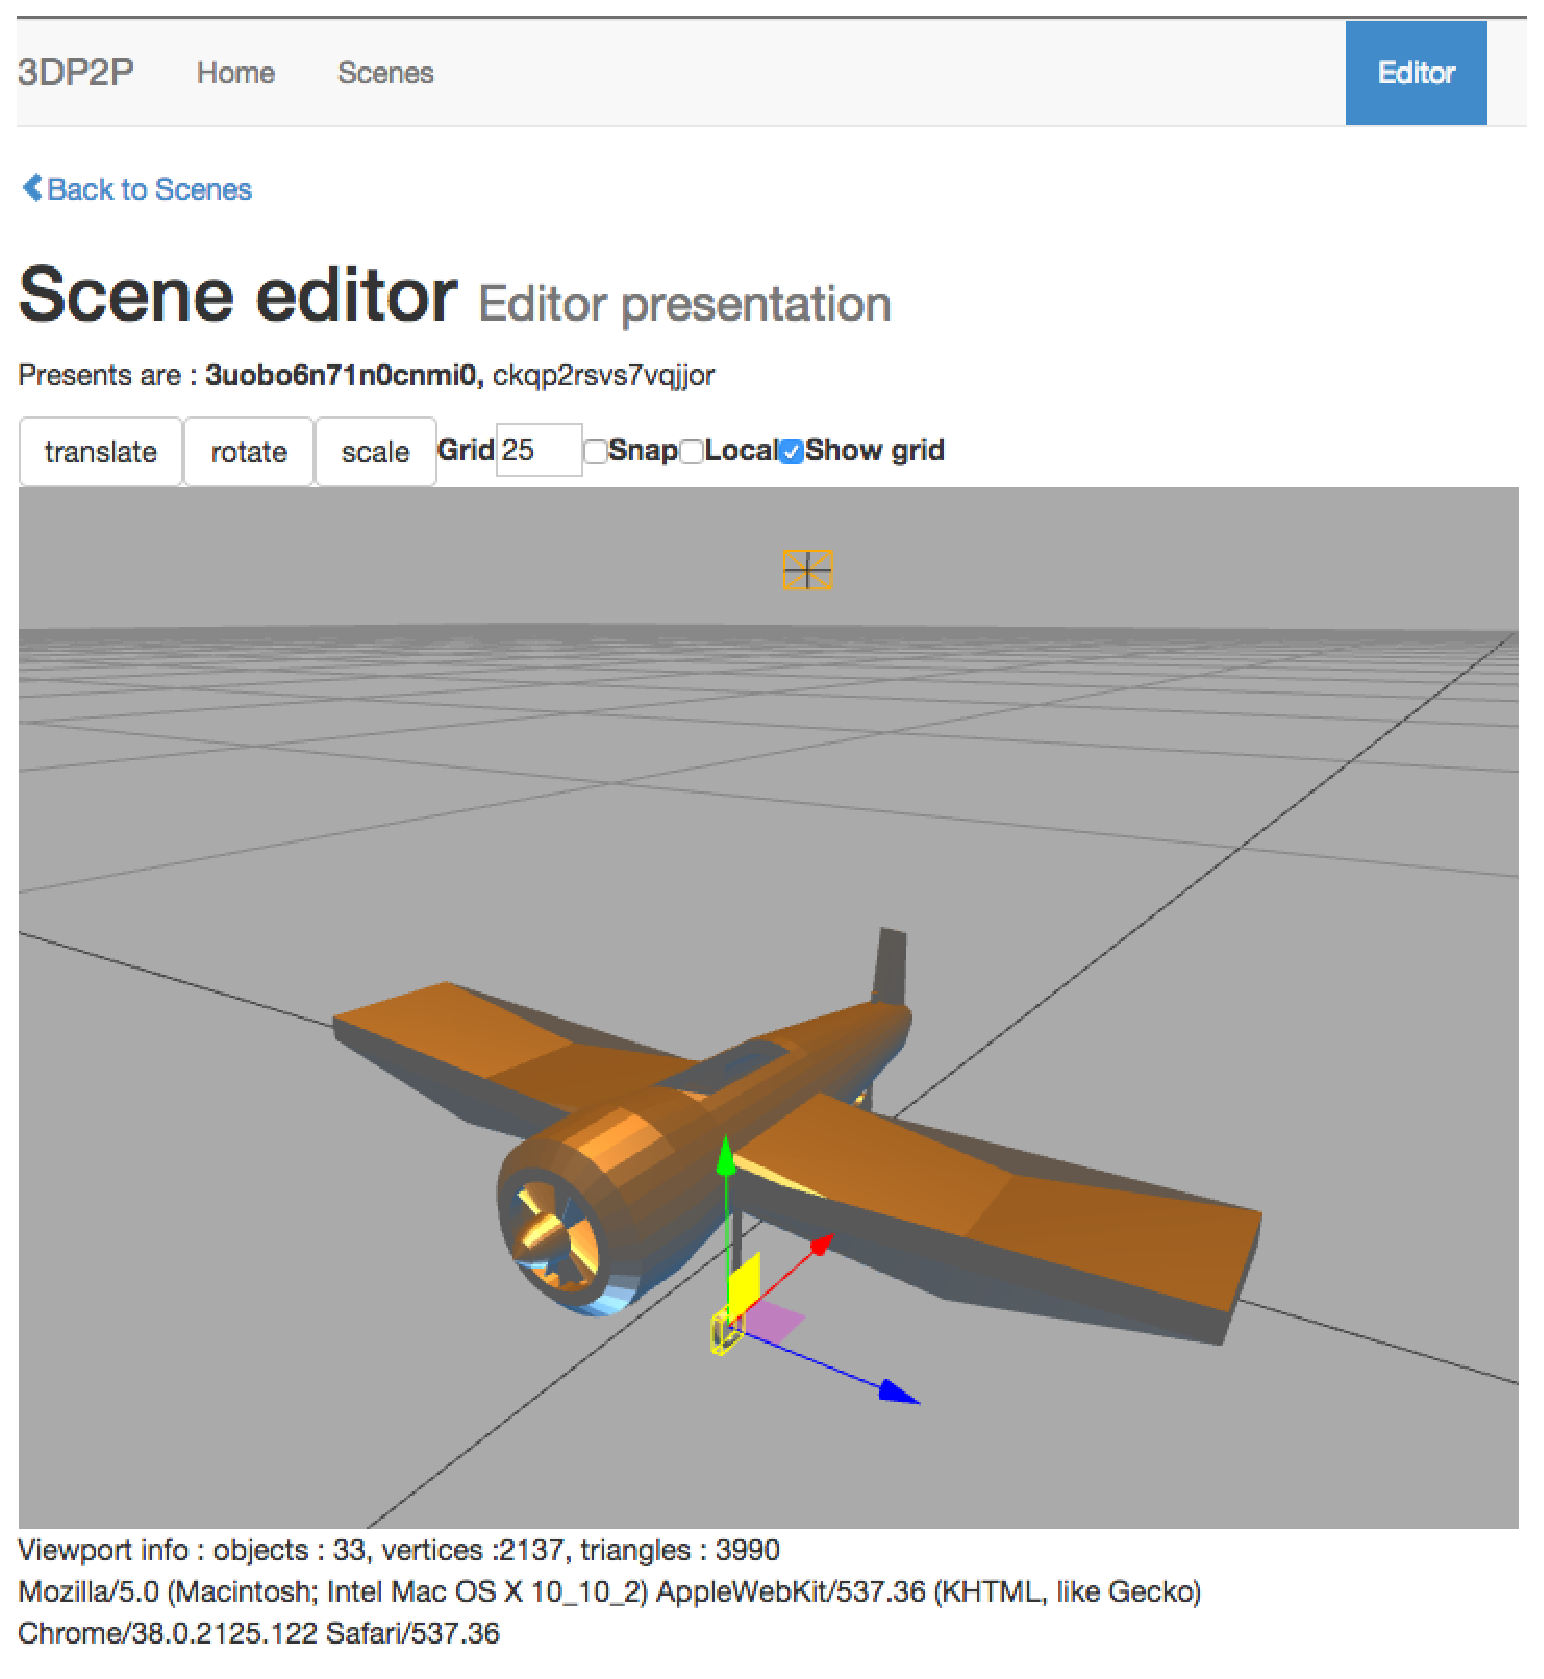
\includegraphics[width=0.6\columnwidth]{eps/editorpresentation.eps}
	\caption{Interface de 3DState}
	\label{fig:3Dstateinterface}
\end{figure}

\subsection{Gestion de la session}
\begin{figure}[h]
	\centering
	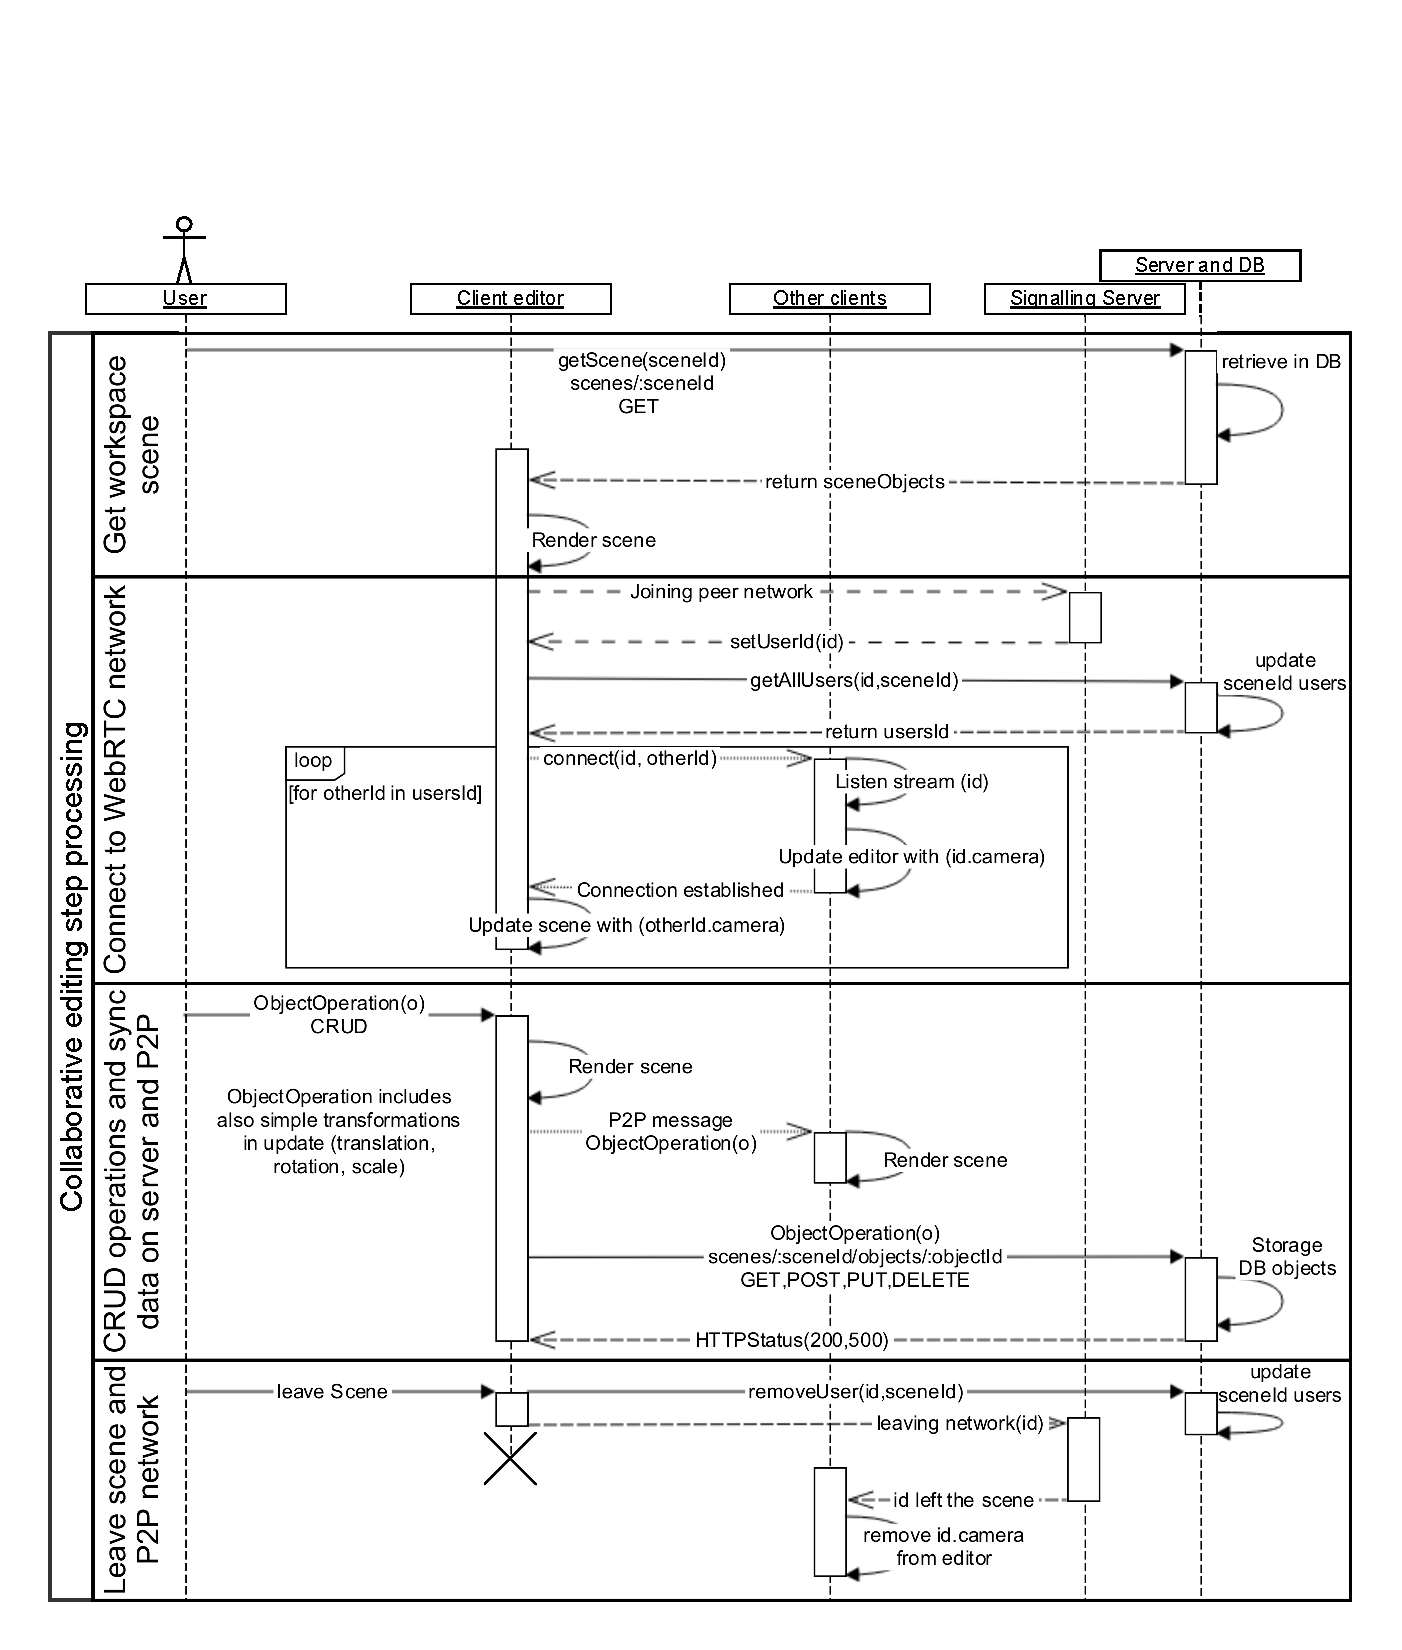
\includegraphics[trim={0 0 0 3cm},clip,width=0.9\columnwidth]
	{eps/sequence_wscg.eps}
	\caption{Diagramme de séquence de la gestion de la session dans une 
		architecture \og orientée état\fg{}}
	\label{fig:sequence_state}
\end{figure}
Lorsqu'un utilisateur rejoint une session, il suit le déroulement des opérations 
décrit dans la Figure \ref{fig:sequence_state}. 
Dans un premier temps, afin de récupérer les données liées à l'espace de travail, 
le client web de l'utilisateur qui se rend sur une scène récupère 
tous les objets associés à la scène dans la base de données. Les objets de la 
scène sont renvoyés à l'éditeur pour les afficher. 
Dans un second temps, le système établit les connexions \gls{P2P} entre les 
clients de manière automatique et complète (topologie réseau en maillage 
complet) après avoir récupéré les identifiants des autres utilisateurs auprès du 
serveur de \textit{signaling}. Une fois la connexion établie, chaque collaborateur 
voit son environnement \gls{3D} dans l'éditeur mis à jour, indiquant la position du 
nouvel 
arrivant. Les collaborateurs éditent ensuite la scène \gls{3D} qui produit, sur les 
différents objets, des requêtes \gls{CRUD} -- incluant les opérations de translation, 
rotation et homothétie -- destinées au serveur (qui transmet les 
modifications à la base de données) puis aux collaborateurs.
Enfin, dans un dernier temps, lorsque l'utilisateur quitte la scène, il en notifie le 
serveur de \textit{signaling} qui s'occupe d'indiquer aux clients restants l'abandon 
du client pour qu'ils puissent mettre à jour leur interface en conséquence.



		
		\subsection{Bilan critique}
Le prototype 3DState est issu de l'implantation de \cite{Desprat2015a} qui 
présente une architecture de communication hybride pour la modélisation 3D 
collaborative. Ses principales fonctionnalités sont : la mise en relation des clients, 
l'utilisation d'une interface web pour visualiser / ajouter / modifier des modèles 
dans une scène 3D. Chaque scène peut accueillir plusieurs collaborateurs et 
permettre à chacun de voir les modifications en temps réel des autres. La couche 
applicative utilise la programmation événementielle pour que les composants de 
l'application réagissent directement aux modifications des objets dans 
l'environnement 3D. 

L'implantation naïve que propose ce prototype pose plusieurs problèmes. 
D'une part, l'interface étant restreinte au minimum, il manque plusieurs 
fonctionnalités fondamentale pour que la modélisation collaborative s'effectue 
dans un environnement adéquat. Par exemple, il n'y a pas de liste 
des objets présents dans une scène et l'historique de la scène est également 
absent. La sensibilisation à la collaboration est quasiment absente (couleur 
différente par collaborateur) à l'exception de la représentation des collaborateurs 
par leur caméra dans l'environnement 3D. Stocker les éléments 3D par 
leur état impose un mise en mémoire coûteuse et des transferts d'autant plus 
coûteux par RTCDatachannel. Le Tableau \ref{table:3DStateChoixTechniques} 
résume les différents choix techniques effectués dans 3DState. 
		
			
			\begin{table}[!h]
				\centering
\caption{\label{table:3DStateChoixTechniques}Résumé des choix techniques pour 
3DState}
\begin{tabular}{llll}
	& \textbf{Plateforme / Service}& \textbf{Bibliothèque (version)}\\ \hline
	& \begin{tabular}[c]{@{}l@{}}
		Rendu WebGL \\ 
		Gestionnaire d'événements 
	\end{tabular} 	& 
	\begin{tabular}[c]{@{}l@{}}
		Three.JS (r69) \\ 
		signal-js (v1.0.0)
	\end{tabular}\\
	\multirow{-3}{*}{\textbf{Pair}} & WebRTC & PeerJS (v0.3.9)\\ \hline
	& Node.JS (v0.10.32)& ExpressJS (v4.9.0)\\
	& WebSocket & PeerJSServer (N/A) \\
	\multirow{-3}{*}{\textbf{Serveur}} & Base de données NoSQL & MongoDB 
	(v2.6.8) \\ \hline
\end{tabular}
\end{table}
			
			\paragraph{Testabilité}
La testabilité de l'application est nulle car tous les composants sont fortement liés 
entre eux. Cela ne permet pas de tester proprement les différents blocs du 
prototype. La collaboration est compliquée à observer dans un environnement 
implanté comme 3DState car l'approche orientée états ne rend pas compte des 
intentions des utilisateurs.